\chapter{Background Information}
\label{ch:background-information}


\begin{itemize}
    \item Classification problem, methods to solve: log regression, trees, deep learning
    \item How to ealuate quality of classification problem (accuracy, precision, recall, F1)
    \item Word embeddings
    \item RNNs and how to get embeddings from them
\end{itemize}

\section{Classification problem}
Classification is a type of machine learning problem when the task is to identify the category  for each observation in test dataset. On the training phase the categories for each observation are provided, so this task is an instance of supervised learning.

As there is a big variety o classification tasks, a large toolkit of classification algorithms currently exist, among which the following groups are most commonly used: 
\begin{itemize}
 \item Linear classifiers
 \item Support Vector Machines
 \item Decision Trees
 \item Artificial Neural Networks
\end{itemize} 

We will concentrate on the last two.

\subsection{Decision Trees}
Decision threes are used for regression as well as for classification. In decision trees a tree-like model of decisions is used to provide the required output on tree's leaves. An example of decision tree is on fig. \ref{fig:decision-tree} This model is built as a sequence of conditional control statements based on values of different features characterizing input observation. A decision tree is mostly learned using recursive binary splitting technique. In this process on each step an algorithm is aimed to find the best feature and splitting condition to finally come up with the shortest path to the final decision. When a feature set is big, then stopping conditions are put on the decision tree to prevent the model from overfitting. 

\begin{figure}[h]
    \centering
    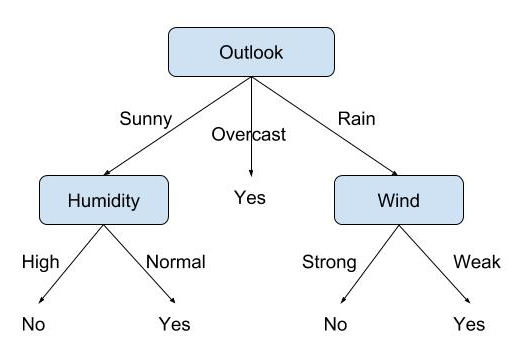
\includegraphics[width=8cm]{Images/Decision-tree.png}
    \caption{A decision tree for decision making about playing tennis on the day.}
    \label{fig:decision-tree}
\end{figure}
% \includegraphics[height=5cm]{Decision tree} 

The advantages of decision trees are:
\begin{itemize}
	\item simplicity of concept and interpretability,
	\item possibility to apply to both categorical and numeric data without a need of regularizaion. 
	\item easiness to combine with other decision techniques.
\end{itemize}

Disadvantages of decision threes are:
\begin{itemize}
	\item instability - a small change in data can lead to dramatic change in model,
	\item propensity of overfitting if no constraints are put.
\end{itemize}


\subsection{Artificial Neural Networks}
\todo{Do we need this section?}

\subsection{Classifier performance evaluation}

To evaluate a classifier the classification results are compared with class labels provided in training dataset. The experimental performance of a classifier on the test data is a proxy for the performance on unseen data. It checks the classifier’s generalization ability.
Binary classifiers are mostly evaluated using confusion matrix (fig. \ref{fig:confusion-matrix}

\begin{figure}[h]
    \centering
    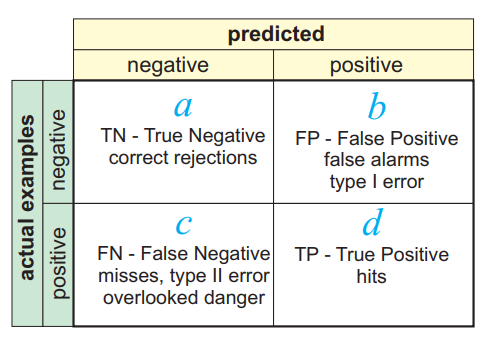
\includegraphics[width=8cm]{Images/Confusion-matrix.png}
    \caption{Confusion matrix. Source: \citep{kohavi:glossary}.}
    \label{fig:confusion-matrix}
\end{figure}

Performance measures calculated from the confusion matrix entries are the following:
\begin{itemize}
    \item Accuracy $= (a + d)/(a + b + c + d) =
    (TN + TP)/total$ ;
    \item True positive rate, recall, sensitivity$ =
    d/(c + d) = TP/actual\: positive$ ;
    \item Specificity, true negative rate $= a/(a + b) =
    TN/actual\: negative$ ; 
    \item Precision, predicted positive value $=
    d/(b + d) = TP/predicted\: positive$ ;
    \item False positive rate, false alarm $= b/(a + b)
    = FP/actual\: negative = 1 - specificity$ ;
    \item False negative rate $= c/(c + d) = FN/actual\: positive$ .
\end{itemize}

One of the measures above is not enough to evaluate a binary classifier properly when data in class imbalanced. For instance, on the examples on fig. \ref{fig:classifiers-evaluation} the accuracy is high and equal for both situations, but precision and recall are highly different. 


\begin{figure}[h]
    \centering
    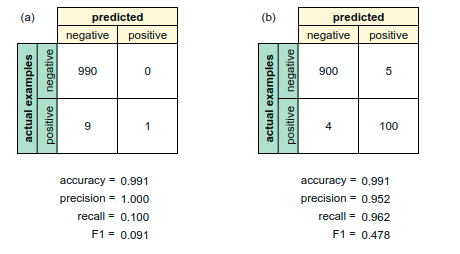
\includegraphics[height=8cm]{Images/Classifiers-evaluation.png}
    \caption{Examples of classifiers evaluation.}
    \label{fig:classifiers-evaluation}
\end{figure}

Moreover, it is always a question what to prioritize, precision or recall, and how to find balance among these two measures. For this reason, $F_1$ score, a harmonic mean of precision and recall, is frequently used to evaluate a binary classifier:

\begin{equation}
    F_{1}=2\cdot {\frac {\mathrm {precision} \cdot \mathrm {recall} }{\mathrm {precision} +\mathrm {recall} }}
\end{equation} 

\section{Vector words representations}

When working with textual data it is a popular approach in machine learning to represent words as vectors, which capture some relationships between words in language.

\subsection{Word2vec}
\todo[inline]{Reformulate next 3 paragraphs ( from  https://www.tensorflow.org/tutorials/representation/word2vec )}
Vector space models (VSMs) represent (embed) words in a continuous vector space where semantically similar words are mapped to nearby points ('are embedded nearby each other'). All methods in VSMs mostly rely on Distributional Hypothesis, which states that words that appear in the same contexts share semantic meaning. The approaches that leverage this principle can be divided into two categories:
\begin{itemize}
    \item count-based methods (e.g. Latent Semantic Analysis), where  the frequency of concurrence with neighboring words in a large text corpus is computed for each word, and then mapped onto a small, dense vector.
    \item redictive methods (e.g. neural probabilistic language models), where each word is predicted out of neighbours by means of learning small, dense embedding vectors, which are actually hidden layer values of a fully connected DNN. 
\end{itemize}

Word2vec is a computationally-efficient predictive model for learning word embeddings from raw text. It can be implemented using two approaches: Continuous Bag-of-Words model (CBOW) and  Skip-Gram model \cite{Mikolov-ICLR2013}. Both of this models are fully connected neural networks aimed to predict words, but CBOW predicts target words (e.g. 'mat') from source context words ('the cat sits on the'), while the skip-gram does the inverse and predicts source context-words from the target words. This inversion might seem like an arbitrary choice, but statistically it has the effect that CBOW smoothes over a lot of the distributional information (by treating an entire context as one observation). For the most part, this turns out to be a useful thing for smaller datasets. However, skip-gram treats each context-target pair as a new observation, and this tends to do better when we have larger datasets. 

A nice property of Word2vec words representation is that due to the way it is learned, final vectors capture context information of words. For this reason such vectors are frequently used as features for many canonical NLP prediction tasks, such as part-of-speech tagging, named entity recognition \citep{Collobert:DBLP}, or classification.


\subsection{Representations from RNN}
\todo{Not sure about the content of this section for now}